% This is a basic Math Paper

\documentclass[11pt]{article}

% Preamble

\usepackage[margin=1in]{geometry}
\usepackage{amsfonts, amsmath, amssymb}
\usepackage{fancyhdr, float, graphicx}
\usepackage[utf8]{inputenc} % Required for inputting international characters
\usepackage[T1]{fontenc} % Output font encoding for international characters
\usepackage{fouriernc} % Use the New Century Schoolbook font
\usepackage[nottoc, notlot, notlof]{tocbibind}
\usepackage[hidelinks]{hyperref}

% Header and Footer
\pagestyle{fancy}
\fancyhead{}
\fancyfoot{}
\fancyhead[L]{\textit{\Large{Trial on Reciprocating Compressor}}}
%\fancyhead[R]{\textit{something}}
\fancyfoot[C]{\thepage}
\renewcommand{\footrulewidth}{1pt}

\begin{document}
	
	\begin{titlepage} 
		\centering 
		
		%---------------------------NAMES-------------------------------
		
		\huge\textsc{
			MIT World Peace University
		}\\
	
		\vspace{0.75\baselineskip} % space after Uni Name
		
		\LARGE{
			Basic Mechanical Engineering\\
			First Year B. Tech, Trimester 1
		}
		
		\vfill % space after Sub Name
		
		%--------------------------TITLE-------------------------------
		
		\rule{\textwidth}{1.6pt}\vspace*{-\baselineskip}\vspace*{2pt}
		\rule{\textwidth}{0.6pt}
		\vspace{0.4\baselineskip} % Whitespace above the title
		
		
		
		\huge{\textsc{
				Trial on Reciprocating Compressor
			}} \\
		
		
		
		\vspace{0.5\baselineskip} % Whitespace below the title
		\rule{\textwidth}{0.6pt}\vspace*{-\baselineskip}\vspace*{2.8pt}
		\rule{\textwidth}{1.6pt}
		
		\vspace{1\baselineskip} % Whitespace after the title block

		%--------------------------SUBTITLE --------------------------	
			
		\LARGE\textsc{
			Experiment Number 7\\Practical Report
		} % Subtitle or further description
		\vfill
		
		%--------------------------AUTHOR-------------------------------
		
		Prepared By
		\vspace{0.5\baselineskip} % Whitespace before the editors
		
		\Large{
			Krishnaraj Thadesar \\
			Division 9, Roll No. 54
		}
		
		
		\vspace{0.5\baselineskip} % Whitespace below the editor list
		\today

	\end{titlepage}
	
	
\tableofcontents
\thispagestyle{empty}
\clearpage


\setcounter{page}{1}

\section{Objective}
To calculate the compression ratio for the reciprocating Air-compressor



\section{Theory}

In two stages compressor air is partially compressed in low-pressure cylinder this air is
passed through between the first stage and the second stage so that air at the inlet of the second stage is
at lower temperature than the first stage outlet. This is done to reduce the work of compressor in second
stage. Final compression is completed in the second stage. Also the compressors are provided with
clearance volume, two stage compressors can achieve higher volumetric efficiency than a single stage
compressor because of lower compression per stage. As the compressed air is used in a wide range in industrial, domestic, aeronautics Fields, etc. so compressors are applied in a wide range. Compressors
are used where the air is required at high pressure



\subsection{About the Compressor}

An Air compressor is a device, which sucks the air from the atmosphere
and compresses it and delivers it to a reservoir tank. It compresses the air by the means of a
reciprocating piston, which reciprocates inside a cylinder. It can be single stage or multi stage. It can be
single acting or double acting. Two-stage air compressor test rig consists of two cylinders and pistons
and a reservoir tank. An A.C motor drives it. Thermometers are provided at inlets and outlets. To find
out the inlet volume of air an orifice is provided. To stream line the intake a diaphragm base manifold is
provided. Pressure gauge is provided at reservoir tank. Safety valve and auto power switch is provided
for the safety factor.


\subsection{Specifications of the Compressor}


\begin{figure}[H]
	\centering
	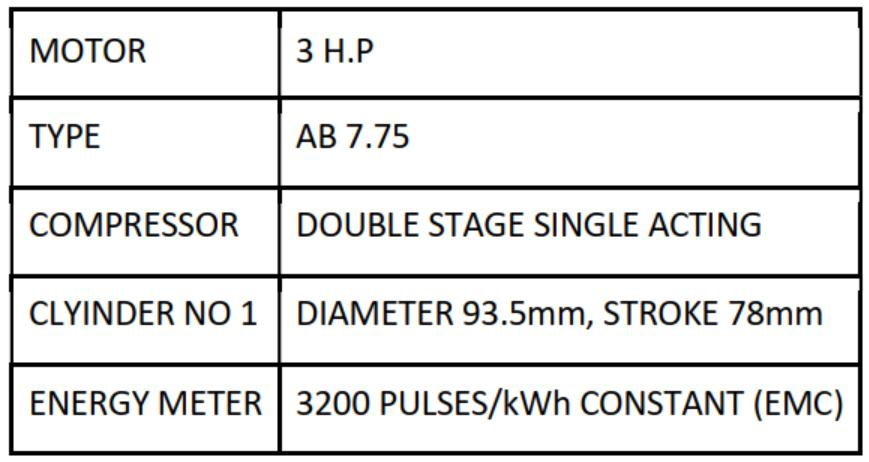
\includegraphics[scale=0.3]{specs.jpg}
\end{figure}


\subsection{Utilities Required}

The four processes in a theoretical Vapour Compression Cycle are:
\parindent 0ex

A. Electric Supply: Single Phase 220V AC, 50 Hz\\
B. Space Required: 2.5 * 1.5 * 3.0 m 

\begin{figure}[H]
	\centering
	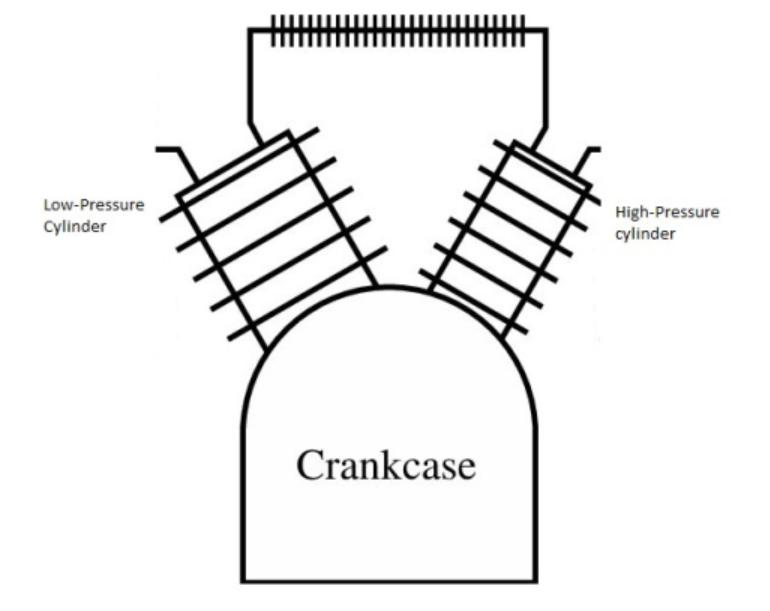
\includegraphics[scale=0.3]{compressor.jpg}
	\caption{Basic Components of a reciprocating compressor}
\end{figure}


\section{Procedure}

\begin{enumerate}
	\item Close the outlet valve of tank and start compressor
	\item Let the receiver pressure rise up to 2 Kg/cm2, now open the delivery valve so that constant delivery pressure is achieved
	\item Wait for some time and see that delivery pressure remains constant, now note down the pressure.
	\item Record the energy meter pulses/time to find out the input power.
	\item Record the manometer reading to find out the volume of air input.
	\item Record the temperature of inlet and before second stage and after second stage
	\item Find out the rpm of compressor with the help of rpm indicator.
	\item Find out the volumetric efficiency and isothermal power by given formulae
	\item Repeat the procedure for different delivery pressures
	
\end{enumerate}

\section{Conclusion}

The compression ratio of compressor is given by:

\centering

\begin{figure}[H]
	\centering
	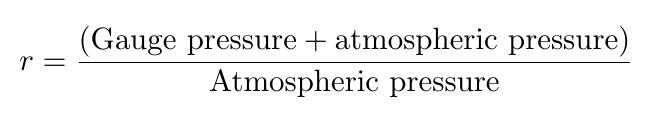
\includegraphics[scale=0.4]{equation.jpg}
\end{figure}


\end{document}